\documentclass[9pt,a4paper,twoside]{tau}
\usepackage[english]{babel}
\usepackage{tauenvs}

%----------------------------------------------------------
% TITLE
%----------------------------------------------------------

\title{Investigative Report of Franklin Resources Inc. [stock: BEN] from April 2022 to April 2024}

%----------------------------------------------------------
% AUTHORS, AFFILIATIONS AND PROFESSOR
%----------------------------------------------------------

\author[a,1]{Bucsa, Justin}

%----------------------------------------------------------

\affil[a]{Stealth}
\professor{}

%----------------------------------------------------------
% FOOTER INFORMATION
%----------------------------------------------------------

\institution{Stealth}
\ftitle{}
\date{April 19, 2024}
\etal{Bucsa}
\course{}

%----------------------------------------------------------
% ABSTRACT
%----------------------------------------------------------

\begin{abstract}    
    This report comprehensively analyzes Franklin Resources Inc. (BEN) as a potential investment opportunity. It examines the company’s performance over two years (April 2022 - April 2024), encompassing historical background, strategic goals, and significant shareholder structure. We will delve into market data to understand BEN’s price movements and analyze key events that transpired within the past year (April 2023 - April 2024) to assess their impact. Finally, the report culminates in a holistic evaluation of Franklin Resources Inc.’s investment potential.
\end{abstract}
%----------------------------------------------------------
% \keywords{}
%----------------------------------------------------------
\begin{document}	
	\maketitle
	\thispagestyle{firststyle}
	\tauabstract
	% \tableofcontents
%----------------------------------------------------------
\section{Introduction}

    \taustart{F}ranklin Resources Inc. [NYSE: BEN] is one of the world’s largest investment managers, better known as Franklin Templeton. The company oversees \$1.6 trillion in total assets under management, over 1400 investment professionals in 25 counties, and more than 9000 workers globally. This report will discuss the following topics: the history of Franklin Resources Inc. [NYSE: BEN], recent events, Ownership distribution of stocks, market analysis, and conclusion. The conclusion will explore the value of Franklin Resources Inc.
    [NYSE: BEN] as a short-term and long-term investment choice.
    

\section{History}
    
    Franklin Resources boasts a rich history dating back to 1947, when it began operations in the investment management field. The company initially focused on mutual funds, offering both fixed-income and equity options (growth and value-oriented). Through strategic acquisitions, Franklin has continuously expanded its reach and expertise.\\
    Notable additions include: \\
    - 1992: Templeton, a global investment firm, bringing international investment capabilities.\\
    - 1996: Franklin Mutual Series, further solidifying its mutual fund portfolio.\\
    - 2000 \& 2001: Acquisitions like Franklin Bissett Canadian and Fiduciary Trust International broadened their offerings to include Canadian investment management and trust services.\\
    - 2019-2022: A period of significant expansion, with acquisitions like Benefit Street Partners (alternative credit), Athena Capital Advisors (wealth management), Legg Mason (global investments), O’Shaughnessy Asset Management (quantitative assets), Lexington Partners (alternative investments), and Alcentra (alternative credit).\\
    
    This growth strategy through acquisitions has transformed Franklin Resources into a leading global investment management firm with diverse offerings to meet evolving investor needs.
    
\section{Events}

    \subsection{May 2023 - Acquisition of Putnam Investments Announced}
	
        Franklin Resources Inc. announced a significant acquisition in May 2023, entering into a definitive agreement to acquire Putnam Investments from Great-West Lifeco Inc. (Great-West), a prominent Power Corporation group member. This strategic move strengthens Franklin Templeton’s position in the asset management industry. Great-West and Power Corporation are global insurance, retirement, wealth management, and asset management leaders, aligning well with Franklin Templeton’s existing strengths.

    \subsection{January 2024 - Acquisition of Putnam Investments Completed}
	
        Franklin Resources Inc. completed the acquisition of Putnam Investments, expanding its global footprint and AUM (Assets Under Management). This strategic move solidified Franklin Resources’ leading investment management firm position.
    
    \subsection{Insider Sales}
        Below is a list of insider stock sales from Franklin Resources Inc. executives and the board of directors from 2022-04-20 to 2024-04-20. 
    
            \begin{figure}[H]
                \centering
                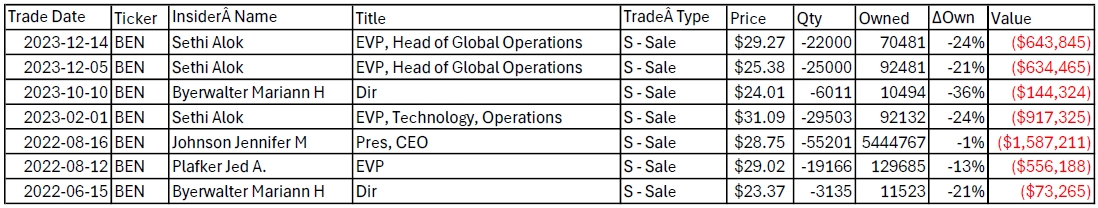
\includegraphics[width=0.95\columnwidth]{images/InsiderTrades.jpg}
                \caption{This is a table of Insider Trades from 2022-04-20 to 2024-04-20.}
                \label{fig:figure}
            \end{figure}
        The noted sales do not seem to have effected the stock price much on the date of sales. 
        
\section{Ownership Distribution}
    \subsection{Breakdown}
        
        Total ownership of Franklin Resources Inc. [NYSE: BEN] is divided into four categories: Insiders, Mutual Funds, Other Institutional Investors, and Public Companies and Individual Investors. The pie chart below shows the distribution of ownership: Insiders own the most at 40.88\%, Public Companies and Individual Investors at 25.85\%, Other Institutional Investors at 19.77\%, and Mutual Funds at 13.50\%.

            \begin{figure}[H]
                \centering
                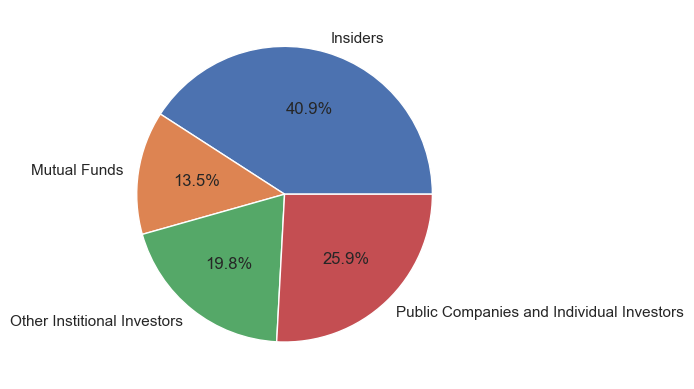
\includegraphics[width=0.85\columnwidth]{images/OwnershipPieChart.png}
                \caption{This chart represents how the shares of BEN are divided up as of 2024-04-20.}
                \label{fig:figure}
            \end{figure}

    \subsection{Concerns}
    
        Franklin Resources Inc. (NYSE: BEN) can be susceptible to immediate stock price swings. With a large portion of the ownership concentrated in insiders, public companies, and other institutional investors (holdings totaling 86.5\%) compared to mutual funds, the stock price could react more dramatically if these major investors decide to sell. This concentration of ownership suggests that BEN might be a more stable choice for short-term investment strategies. Still, the vulnerability to large investor sentiment should be considered for long-term investors.

\section{Market Analysis}
    \subsection{Introduction to Market Analysis}
        
        This section will examine the Closing Price and Quarterly Revenue of Franklin Resources Inc. (NYSE: BEN) from 2022-04-20 to 2024-04-20. We will discuss the possible impacts of each of them and then compare them.
    
    \subsection{Closing Price}
        
        Below is the Closing Cost of Franklin Resources Inc. (NYSE: BEN) per month from 2022-04-20 to 2024-04-20.
            \begin{figure}[H]
                \centering
                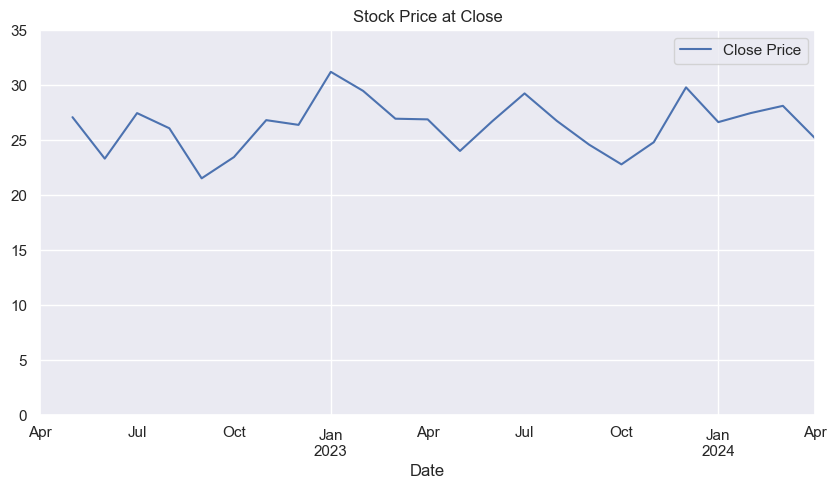
\includegraphics[width=0.85\columnwidth]{images/CloseDataSet1mo.png}
                \caption{This chart represents the Closing Stock Price per Month from 2022-04-20 to 2024-04-20.}
                \label{fig:figure}
            \end{figure}
        
        The price appears to be in a flux of plus or minus \$5.00 every quarter, a rate of change near 16.67\% of the stock value. If we look at the daily trades, we can see the jumps more clearly occur at a quarterly period. 
            \begin{figure}[H]
                \centering
                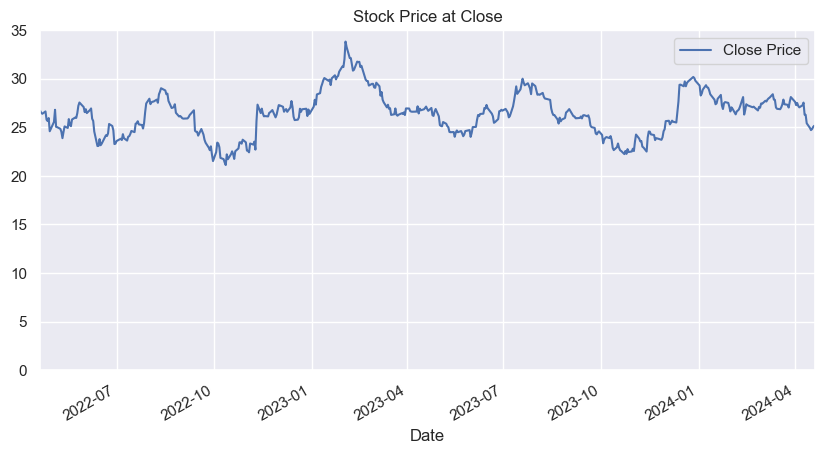
\includegraphics[width=0.85\columnwidth]{images/CloseDataSet1d.png}
                \caption{This chart represents the Closing Stock Price per Day from 2022-04-20 to 2024-04-20.}
                \label{fig:figure}
            \end{figure}
        
        If we compare the two charts, we can see the monthly average trails in the daily report due to these large jumps in the closing price.
            \begin{figure}[H]
                \centering
                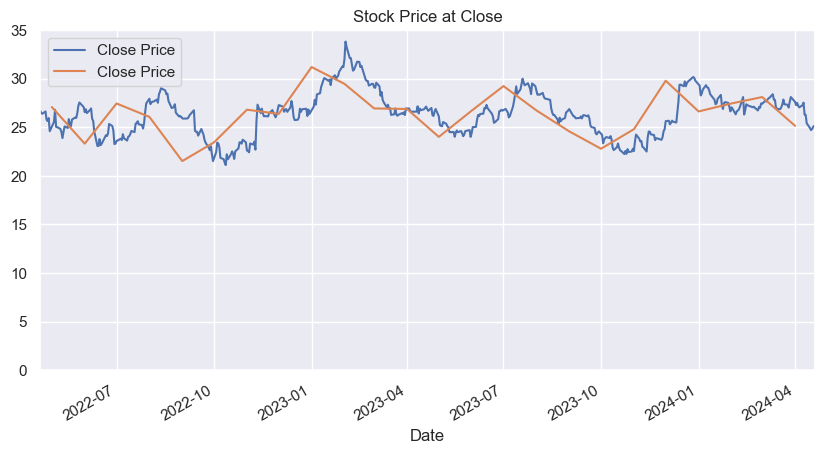
\includegraphics[width=0.85\columnwidth]{images/CloseDataSet1dvs1mo.png}
                \caption{This chart represents the Closing Stock Price per Day vs. Closing Stock Price per Month from 2022-04-20 to 2024-04-20.}
                \label{fig:figure}
            \end{figure}
        
        Thus, we may conclude that a market force acting at the start makes it visible for daily trading over monthly trading.
        
        Let us continue into the Quarterly Revenue reports.
            
    \subsubsection{Quarterly Revenue}
        
        Since Franklin Resources Inc. [NYSE: BEN] has over \$1.6 trillion in assets under management, its earnings report shows a profit of sometimes breaking \$200 billion in the recent quarter. Below is a chart showing the recent Quarter Revenue from 2022-04-20 to 2024-04-20.
            \begin{figure}[H]
                \centering
                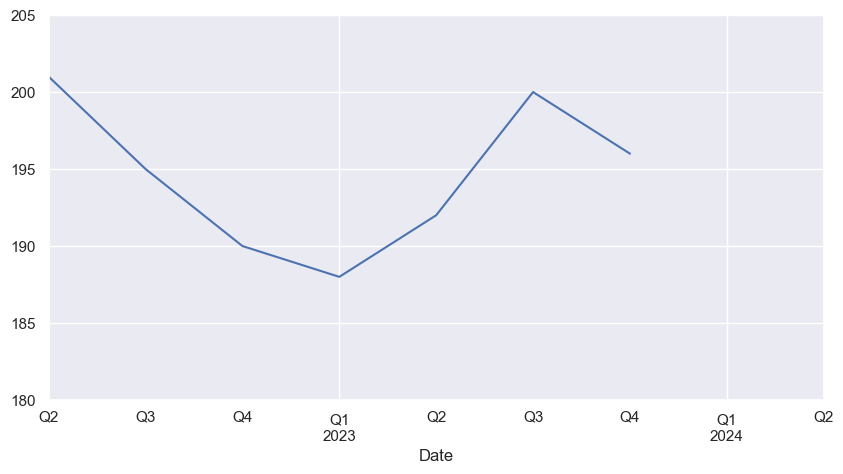
\includegraphics[width=0.85\columnwidth]{images/EarningByQt.png}
                \caption{This chart represents the report earnings in Billions over the quarters from 2022-04-20 to 2024-04-20.}
                \label{fig:figure}
            \end{figure}
        
        It appears that the revenue of Franklin Resources Inc. [NYSE: BEN] does fluctuate plus or minus \$5 billion, coming to a rate of change near 2.5\%. That means the stock value has a rate of change nearly 666.8\% higher than the rate of change in revenue. 
            
    \subsubsection{Closing Price vs. Quarterly Revenue}   
        
        Let us now simply compare the stock's Closing Price to the Quarterly Revenue. We will do this by laying the Quarterly Revenue chart onto the Closing Price chart. Note that the Y-axis to the right is the value of the stock, and the Y-axis to the left is the Gross Revenue value in billions. The x-axis is the same for both.
            \begin{figure}[H]
                \centering
                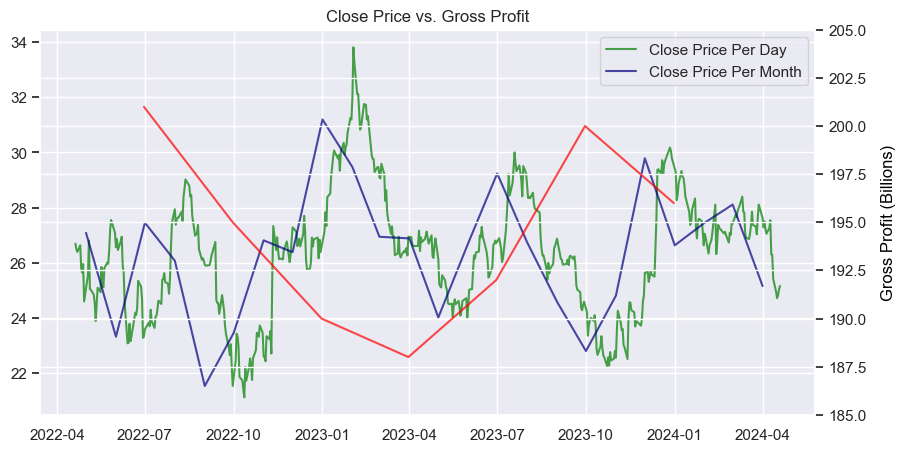
\includegraphics[width=0.85\columnwidth]{images/CloseDataVsProfit.png}
                \caption{This chart compares the monthly and daily closing price against the reported quartly earning price (in red) 2022-04-20 to 2024-04-20.}
                \label{fig:figure}
            \end{figure}
        
        Now, we can see that the change in the stock value is inversely related to the reported revenue. What is causing this?

        Well, in May 2023, the stock rose due to the new merger, but the merger cost impacted the profit then. Thus, investors panicked when the following revenue reports came out, and the stock dropped. However, after the merger, the company was becoming more profitable due to the completion of the merger, but investors still had not returned to the stock. It was not until the following earning report that the investor came back. As of the most recent quarterly report, we see that the profit not being continuously positive negatively impacts the stock value of Franklin Resources Inc. [NYSE: BEN]. Thus, the stock price will be drastically affected if the quarterly report does not exceed \$200 billion in revenue. 



\section{Conclusion}
    \subsubsection{Short Term}
    
        Franklin Resources Inc. [NYSE: BEN] is an active stock with an ideal flux or movement rate for day trading. Even though the stock price appears to be moving in a downward direction, it holds a strong value since the companies report earnings in the \$200 billion mark constantly. Thus, if the stock drops 5\%-10\% in a day, there is a good chance it will recover in a positive direction the following day or even within the same day of trading.

    \subsubsection{Long Term}
    
        It's not the most ideal for long-term investments. Franklin Resources Inc. [NYSE: BEN] appears to rely heavily on acquisitions to remain profitable in the long term. It would be ideal if the short-term investor did not affect value as dramatically as they do. Looking at the most recent dating for the last two years, an investor barely broke even due to fluxation caused by the day trading community. For that, a long-term investment may oversee a 2\% to 5\% return beyond two years. Therefore, no long-term investor should invest in Franklin Resources Inc. [NYSE: BEN] when other S&P stocks have proven much more reliable over the long term.

%----------------------------------------------------------

\addcontentsline{toc}{section}{References}
\printbibliography


%----------------------------------------------------------

\begin{center}

	\textit{Contact:} \\

	\faEnvelope[regular]\ justin.bucsa@gmail.com \\

\end{center}

%----------------------------------------------------------

\end{document}